\chapter{NCC}
Please tell more about conclusion and how to the next work of this study.

\section{Lusia Violita Aprilian-1184080}
\subsection{Teori}
\begin{enumerate}
\item Menjelaskan kenapa file teks harus dilakukan tokenizer
	\par Tokenizer adalah untuk membuat vektor dari teks. Dan mengapa harus dilakukan tokenizer? itu karena dengan memfungsikan tokenizer, teks dapat divektorkan. Sehingga teks yang telah telah divektorkan tersebut dapat terbaca pada Machine Learning.
	\par Berikut adalah ilustrasi pemakaian pada tokenizer, perhatikan gambar \ref{7A1}
		\begin{figure}[!hbtp]
		\centering
		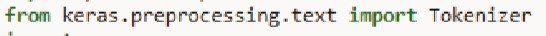
\includegraphics[scale=0.4]{figures/v1.jpg}
		\caption{Lusia-Tokenizer}
		\label{7A1}
		\end{figure}

\item Menjelaskan konsep dasar K-Fold Cross Validation
	\lstinputlisting[firstline=8, lastline=20]{src/1164080/7A2.py}
	\par Berdasarkan kode listing tersebut dapat dijelaskan bahwa :
	\begin{enumerate}
	\item Membuat variabel kfold yang memanggil fungsi StratifiedKFold. StratifiedKFold itu sendiri ialah variasi Kfold yang mengembalikan lipatan bertingkat. Yang dimana pada kode program tersebut jumlah lipatannya adalah 5 atau dibagi menjadi 5 bagian.
	\item Membuat variabel split yang mempresentasikan variabel kfold untuk dibagi berdasarkan class.
	\end{enumerate}
	
	\par Berikut adalah gambar ilustrasi dari kosep dasar kfold, perhatikan gambar \ref{7A2}.
		\begin{figure}[!hbtp]
		\centering
		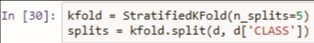
\includegraphics[scale=0.4]{figures/v2.jpg}
		\caption{Lusia-StratifiedKFold}
		\label{7A2}
		\end{figure}

\item Menjelaskan kode program for train, test in splits.
	\lstinputlisting[firstline=8, lastline=20]{src/1164080/7A3.py}
	
	\par Berdasarkan kode program tersebut, maka dapat dijelaskan bahwa kode tersebut digunakan untuk mencetak posisi pengujian pada train dan test yang telah dipisahkan. Dan memastikan bahwa kedua data tersebut tidak terjadi overlaping atau tumpang tindih dalam  setiap pemisahan.
	
	\par Berikut adalah gambar ilustrasi dari for train, test in splits, perhatikan gambar \ref{7A3a}.
	
		\begin{figure}[!hbtp]
		\centering
		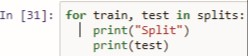
\includegraphics[scale=0.4]{figures/v3a.jpg}
		\caption{Lusia-for train, test in splits}
		\label{7A3a}
		\end{figure}
		
	\par Apabila kode program pada gambar \ref{7A3a} dijalankan, maka akan menghasilkan row\_id sebanyak 5 bagian. Dan jika diperthatikan, setiap bagian tidak terjadi pengulangan sehingga bisa bisa dibilang tidak terjadi overlaping pada data. Perhatikan gambar \ref{7A3b}.
		\begin{figure}[!hbtp]
		\centering
		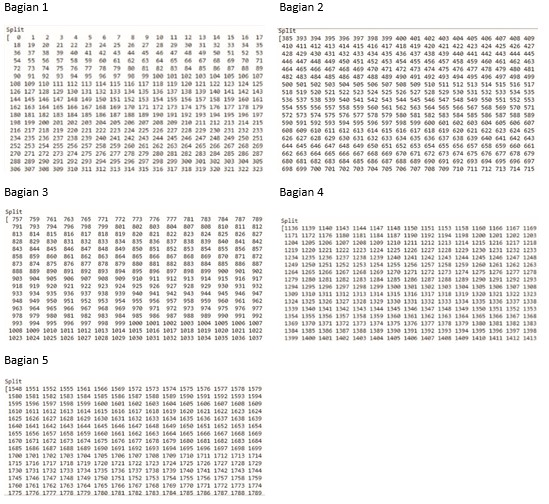
\includegraphics[scale=0.3]{figures/v3b.jpg}
		\caption{Lusia-Hasil Bagian 1}
		\label{7A3b}
		\end{figure}

\item Menjelaskan maksud kode program
	\lstinputlisting[firstline=8, lastline=20]{src/1164080/7A4.py}
	\par Dari kode program tersebut dapat dijelaskan bahwa membuat fungsi train dan test dengan menggunakan dataset yang hanya diambil kolom 'CONTENT' saja. iloc berfingsi sebagai pengindeksan posisi menggunakan integer.
	
	\par Berikut ilustrasi dari kode program tersebut, perhatikan gambar \ref{7A4}.
		\begin{figure}[!hbtp]
		\centering
		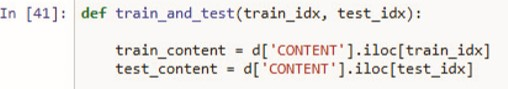
\includegraphics[scale=0.4]{figures/v4.jpg}
		\caption{Lusia-Ilustrasi Kode Program No.4}
		\label{7A4}
		\end{figure}

\item Menjelaskan maksud fungsi
	\lstinputlisting[firstline=8, lastline=20]{src/1164080/7A5.py}
		
	\par Dari kode program tersebut dapat dijelaskan bahwa pada baris pertama adalah membuat variabel tokenizer untuk memanggil fungsi tokenizer agar dapat dilakukan vektorisasi dari kata. Dimana pada kode program pada baris pertama menggunakan 2000 kata atau 2000 kolom.
	\par Sedangkan pada baris kedua dari kode program tersebut menjelaskan bahwa tokenizer difungsikan pada data train yang telah di fitting.
	
	\par Berikut adalh gambar ilustrasi dari fungsi pada kode program tersebut, perhatikan gambar \ref{7A5}.
	
		\begin{figure}[!hbtp]
		\centering
		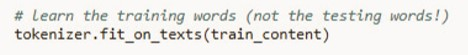
\includegraphics[scale=0.4]{figures/v5.jpg}
		\caption{Lusia-Ilustrasi Maksud fungsi No.5}
		\label{7A5}
		\end{figure}

\item Menjelaskan maksud fungsi
	\lstinputlisting[firstline=8, lastline=20]{src/1164080/7A6.py}
		
	\par Dari fungsi pada kode program tersebut dapat dijelaskan bahwa :
	\begin{enumerate}
	\item Baris pertama membuat variabel d\_train\_inputs untuk memanggil fungsi tokrnizer dan merubah data train yang berupa teks ke dalam bentuk matrix dengan menggunakan model tfidf.
	\item Baris kedua membuat variabel d\_test\_inputs untuk memanggil fungsi tokrnizer dan merubah data test yang berupa teks ke dalam bentuk matrix dengan menggunakan model tfidf.
	\end{enumerate}
	
	\par Berikut adalah gambar ilustrasi dari fungsi pada kode program tersebut, perhatikan gambar \ref{7A6}.
	
		\begin{figure}[!hbtp]
		\centering
		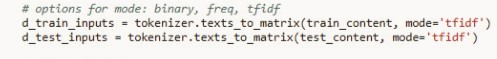
\includegraphics[scale=0.4]{figures/v6.jpg}
		\caption{Lusia-Ilustrasi Maksud fungsi No.6}
		\label{7A6}
		\end{figure}
		
\item Menjelaskan maksud fungsi
	\lstinputlisting[firstline=8, lastline=20]{src/1164080/7A7.py}
		
	\par Dari fungsi pada kode program tersebut dapat dijelaskan bahwa fungsi tersebut akan membagi matrix tfidf tadi dengan amax yaitu mengembalikan maksimum array atau maksimum sepanjang sumbu. Yang hasilnya akan dimasukan kedalam variabel d\_train\_inputs untuk data train dan d\_test\_inputs untuk data test dengan nominal absolut atau tanpa ada bilangan negatif dan koma.
	
	\par Berikut adalah gambar ilustrasi dari fungsi pada kode program tersebut, perhatikan gambar \ref{7A7}.
	
		\begin{figure}[!hbtp]
		\centering
		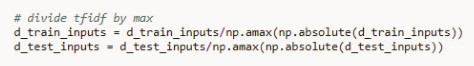
\includegraphics[scale=0.4]{figures/v7.jpg}
		\caption{Lusia-Ilustrasi Maksud fungsi No.7}
		\label{7A7}
		\end{figure}
	
\item Menjelaskan maksud fungsi
	\lstinputlisting[firstline=8, lastline=20]{src/1164080/7A8.py}
		
	\par Dari fungsi pada kode program tersebut dapat dijelaskan bahwa fungsi tersebut ditujukan untuk melakukan one-hot encoding supaya bisa masuk dan digunakan pada neural network. One-hot encoding diambil dari 'CLASS' yang berarti hanya terdapat 2 neuron, yaitu satu nol(1,0) atau nol satu(0,1) karena pilihannya hanya ada dua (spam atau bukan).
	\par Berikut adalah gambar ilustrasi dari fungsi pada kode program tersebut, perhatikan gambar \ref{7A8}.
		\begin{figure}[!hbtp]
		\centering
		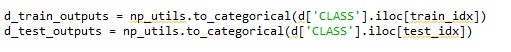
\includegraphics[scale=0.4]{figures/v8.jpg}
		\caption{Lusia-Ilustrasi Maksud fungsi No.8}
		\label{7A8}
		\end{figure}

\item Menjelaskan maksud fungsi
	\lstinputlisting[firstline=8, lastline=20]{src/1164080/7A9.py}
	\par Dari fungsi pada kode program tersebut ditujukan untuk melakukan pemodelan dengan sequential, membandingkan setiap satu larik elemen dengan cara satu persatu secara beruntun. Dimana terdapat 512 neuron inputan dengan input shape 2000 vektor yang sudah dinormalisasi. Lalu model dilakukan aktivasi dengan fungsi 'relu'. Kemudian dilakukan pemotongan bobot supaya tidak overfitting sebesar 50 persen dari neuron inputan 512. Lalu pada layer output terdapat 2 neuron outputan yaitu nol(1,0) atau nol satu(0,1). Kemudian outputan tersebut diaktivasi menggunakan fungsi softmax (mencari nilai maximal).
	\par Berikut adalah gambar ilustrasi dari fungsi pada kode program tersebut, perhatikan gambar \ref{7A9}.
		\begin{figure}[!hbtp]
		\centering
		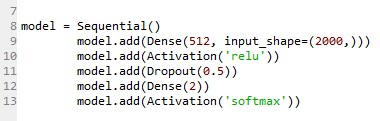
\includegraphics[scale=0.4]{figures/v9.jpg}
		\caption{Lusia-Ilustrasi Maksud fungsi No.9}
		\label{7A9}
		\end{figure}
		
\item Menjelaskan maksud fungsi
	\lstinputlisting[firstline=8, lastline=20]{src/1164080/7A10.py}
	\par Dari fungsi pada kode program tersebut model yang telah dibuat selanjutnya dicompile dengan menggunakan algoritma optimisasi, fungsi loss, dan fungsi metrik.
	\par Berikut adalah gambar ilustrasi dari fungsi pada kode program tersebut, perhatikan gambar \ref{7A10}.
		\begin{figure}[!hbtp]
		\centering
		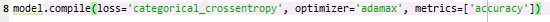
\includegraphics[scale=0.4]{figures/v10.jpg}
		\caption{Lusia-Ilustrasi Maksud fungsi No.10}
		\label{7A10}
		\end{figure}

\item Menjelaskan apa itu Deep Learning
	\par Deep Learning merupakan cabang dari Machine Learning atau bagian keluarga yang lebih luas dari method machine learning berdasarkan pada representasi data pembelajaran. Deep Learning menggunakan Deep Neural Network dalam menyelesaikan suatu masalah yang terjadi pada Machine Learning.
	
\item Menjelaskan apa itu Deep Neural dan bedanya dengan Deep Learning
	\par Deep Neural Network atau DNN merupakan algoritma yang berbasis neural network yang digunakan untuk mengambil keputusan.
	\par Yang membedakan Deep Learning dengan  Deep Neural Network (DNN) adalah DNN merupakan algoritma yang digunakan pada Deep Learning, sedangkan Deep Learning merupakan model yang menggunakan algoritma DNN.
	
\item Menjelaskan perhitungan algoritma konvolusi
	\par Konvolusi pada sebuah gambar dilakukan dalam image processing untuk menerapkan operator yang mempunyai nilai output dari piksel gambar yang berasal dari kombinasi linear nilai input piksel tertentu pada gambar. 
	\par Karena NPM saya 1164080 dan hasil dari (NPM mod 3)+1 = 3, maka saya menggunaan matrik kernel berukuran 3x3. Sehingga ilustrasi gambar yang digunakan adalah seperti gambar \ref{7A13}. Misalkan  f(x,y) yang digunakan berukuran 5x5 dan kernel atau mask berukuran 3x3 masing-masing adalah sebagai berikut: 
		\begin{figure}[!hbtp]
		\centering
		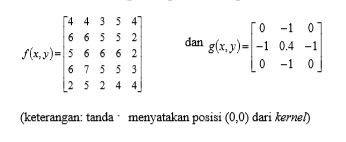
\includegraphics[scale=0.4]{figures/v13.jpg}
		\caption{Lusia-Ilustrasi Gambar}
		\label{7A13}
		\end{figure}
	\par Penyelesaian dari operasi konvolusi antara  f(x,y) dengan kernel g(x,y) pada gambar \ref{7A13} adalah  f(x,y) * g(x,y) dengan ilustrasi sebagai berikut :
	\begin{enumerate}
	\item Tempatkan matrik kernel di sebelah kiri atas, lalu hitung nilai piksel pada posisi (0,0) dari kernel tersebut seperti gambar \ref{7A13a}.
		\begin{figure}[!hbtp]
		\centering
		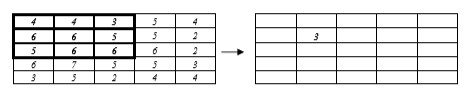
\includegraphics[scale=0.4]{figures/v13a.jpg}
		\caption{Lusia-Ilustrasi konvolusi 1}
		\label{7A13a}
		\end{figure}
		\par Konvolusi dihitung dengan cara berikut :
		\par (0x4) + (-1x4) + (0x3) + (-1x6) + (4x6) + (-1x5) + (0x5) + (-1x6) + (0x6)
		\par Sehingga didapat hasil konvolusi = 3
	\item Lalu geser kernel satu piksel ke kanan kemudian hitung kembali  nilai piksel pada posisi (0,0) dari kernel.
	\par Konvolusi dihitung dengan cara berikut :
	\par (0x4) + (-1x3) + (0x5) + (-1x6) + (4x5) + (-1x5) + (0x6) + (-1x6) + (0x6)  
	\par Sehingga didapat hasil konvolusi = 0 seperti pada gambar \ref{7A13b}.
		\begin{figure}[!hbtp]
		\centering
		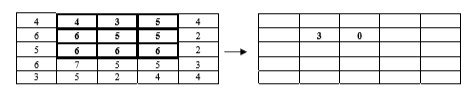
\includegraphics[scale=0.4]{figures/v13b.jpg}
		\caption{Lusia-Ilustrasi konvolusi 2}
		\label{7A13b}
		\end{figure}
		
	\item Lalu geser kernel satu piksel ke kanan kemudian hitung kembali  nilai piksel pada posisi (0,0) dari kernel.
	\par Konvolusi dihitung dengan cara berikut :
	\par (0x3) + (-1x5) + (0x4) + (-1x5) + (4x5) + (-1x2) + (0x6) + (-1x6) + (0x2)  
	\par Sehingga didapat hasil konvolusi = 2 seperti pada gambar \ref{7A13c}.
		\begin{figure}[!hbtp]
		\centering
		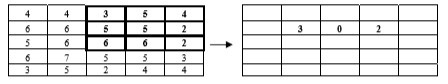
\includegraphics[scale=0.4]{figures/v13c.jpg}
		\caption{Lusia-Ilustrasi konvolusi 3}
		\label{7A13c}
		\end{figure}
		
	\item Kemudian geser matriks kernel kebawah, lalu mulai hitung kembali dari sisi kiri. Setiap kali perhitungan konvolusi dilakukan, geser matriks kernel atau piksel ke kanan seperti pada gambar \ref{7A13d}, \ref{7A13e}, dan \ref{7A13f}.
	\begin{itemize}
	\item Konvolusi pada gambar \ref{7A13d} dihitung dengan cara berikut :
	\par (0x6) + (-1x6) + (0x5) + (-1x5) + (4x6) + (-1x6) + (0x6) + (-1x7) + (0x5)   
	\par Sehingga didapat hasil konvolusi = 0 seperti pada gambar \ref{7A13d}.
		\begin{figure}[!hbtp]
		\centering
		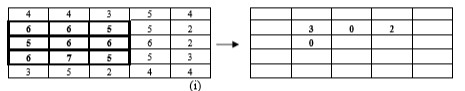
\includegraphics[scale=0.4]{figures/v13d.jpg}
		\caption{Lusia-Ilustrasi konvolusi 4}
		\label{7A13d}
		\end{figure}
	\item Konvolusi pada gambar \ref{7A13e} dihitung dengan cara berikut :
	\par (0x6) + (-1x5) + (0x5) + (-1x6) + (4x6) + (-1x6) + (0x7) + (-1x5) + (0x5)   
	\par Sehingga didapat hasil konvolusi = 2 seperti pada gambar \ref{7A13e}.
		\begin{figure}[!hbtp]
		\centering
		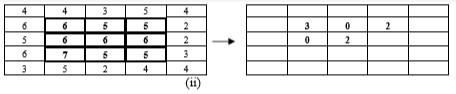
\includegraphics[scale=0.4]{figures/v13e.jpg}
		\caption{Lusia-Ilustrasi konvolusi 5}
		\label{7A13e}
		\end{figure}
		
	\item Konvolusi pada gambar \ref{7A13f} dihitung dengan cara berikut :
	\par (0x5) + (-1x5) + (0x2) + (-1x6) + (4x6) + (-1x2) + (0x5) + (-1x5) + (0x3)    
	\par Sehingga didapat hasil konvolusi = 6 seperti pada gambar \ref{7A13f}.
		\begin{figure}[!hbtp]
		\centering
		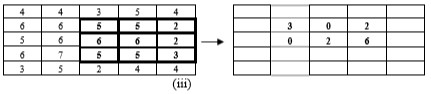
\includegraphics[scale=0.4]{figures/v13f.jpg}
		\caption{Lusia-Ilustrasi konvolusi 6}
		\label{7A13f}
		\end{figure}
	\end{itemize}		
	\item Dengan langkah-langkah yang sama, piksel-piksel pada baris ketiga dilakukan orerasi konvolusi sehingga menghasilkan seperti gambar \ref{7A13g}.
		\begin{figure}[!hbtp]
		\centering
		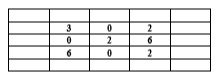
\includegraphics[scale=0.4]{figures/v13g.jpg}
		\caption{Lusia-Ilustrasi konvolusi baris ketiga}
		\label{7A13g}
		\end{figure}
	\par Apabila nilai piksel hasil konvolusi adalah negatif, maka nilai tersebut dijadikan 0. Sebaliknya, bila nilai piksel hasil konvolusi lebih besar dari nilai kabuan maksimum (255), maka nilai tersebut dijadikan ke nilai keabuan maksimum.
	
	\end{enumerate}

\end{enumerate}

\subsection{Cek Plagiarisme}
\par Dari hasil kerja pada chapter 7, jika dicek plagiarisme menghasilkan seperti gambar \ref{7D1}.
		\begin{figure}[!hbtp]
		\centering
		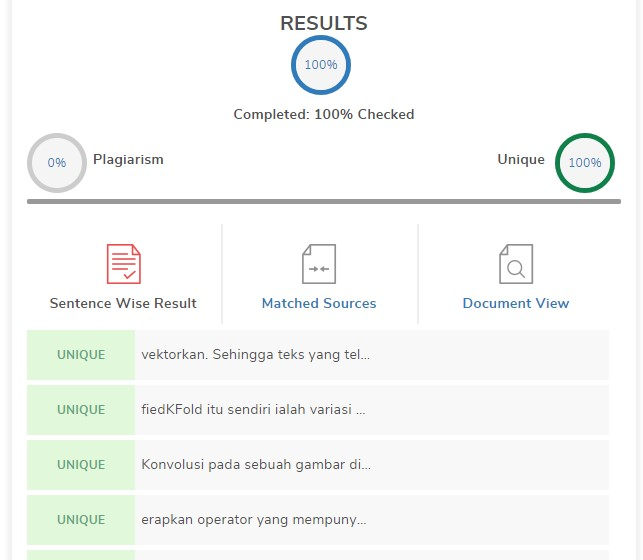
\includegraphics[scale=0.4]{figures/pc7.jpg}
		\caption{Lusia-Plagiarisme}
		\label{7D1}
		\end{figure}



\par
\par
\par
\par
\section{Fadila-1164072}
\subsection{Teori}
Penjelasan Tugas Harian 12 ( No 1-11 ).
\begin{enumerate}
\item Mengapa File Teks Harus Dilakukan Tokenizer Besera Ilustrasi Gambar :
\begin{itemize}
\item Tokenizer :
\par Difungsikan untuk membuat vektor dari text. Lebih detailnya, tokenizer merupakan langkah pertama yang diperlukan dalam banyak tugas pemrosesan bahasa alami, seperti penghitungan kata, penguraian, pemeriksaan ejaan, pembuatan corpus, dan analisis statistik teks.
\par
\par
\item Mengapa Text Harus Dilakukan Tokenizer ? :
\par Text harus dilakukan tokenizer agar dapat dirubah menjadi vektor. Dari perubahan ke vektor tersebut maka data/textnya dapat dibaca oleh komputer (terkomputerisasi).
\par
\par
\item Ilustrasi Gambar : \ref{chapter-7-tokenizer-fadila}
\par
\begin{figure}[!hbtp]
\centering
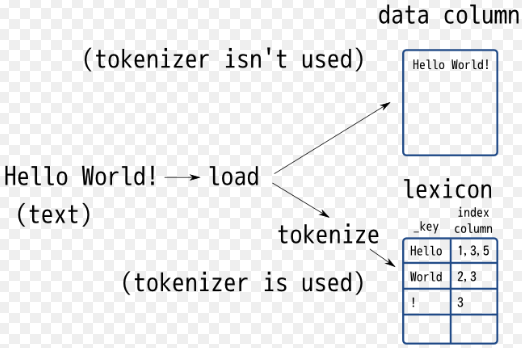
\includegraphics[scale=0.2]{figures/chapter-7-tokenizer-fadila.png}
\caption{Tokenizer - fadila}
\label{chapter-7-tokenizer-fadila}
\end{figure}
\par
\end{itemize}
\par
\par
\item Konsep Dasar K Fold Cross Validation Pada Dataset Komentar Youtube Pada Kode Listing Beserta Dengan Ilustrasi Gambar :
\item Jelaskan Apa Maksud Kode Program For Train Dan Test In Splits Dilengkapi Dengan Ilustrasi Gambar :
\item Apa Maksud Kode Program train\_content = d['CONTENT'].iloc[train\_idx] dan test\_content = d['CONTENT'].iloc[test\_idx] Dilengkapi Dengan Ilustrasi Gambar :
\item Apa Maksud Dari Fungsi Tokenizer = Tokenizer(num words=2000) Dan Tokenizer.fit on texts(train content), Dilengkapi Dengan Ilustrasi Gambar :
\item Apa Maksud Dari Fungsi d train inputs = tokenizer.texts to matrix(train content, mode=’tfidf ’) dan d test inputs = tokenizer.texts to matrix(test content, mode=’tfidf ’), Dilengkapi Dengan Ilustrasi Kode Dan Atau Gambar :
\item Apa Maksud Dari Fungsi d train inputs = d train inputs/np.amax(np.absolute(d\_train) :
\item Apa Maksud Dari Fungsi Di Listing ?? Dengan Parameter Tersebut. [caption=Compile model,label=lst:7.2] model.compile(loss=’categoricalcrossentropy0, optimizer =0 adamax0, metrics = [0accuracy0]) :
\par
\item Apa itu Deep Learning :
\begin{itemize}
\item Penjelasan :
\par Deep learning merupakan sub bidang pembelajaran mesin yang berkaitan dengan algoritma yang terinspirasi oleh struktur dan fungsi otak yang disebut jaringan saraf tiruan.
\par
\par
\par
\end{itemize}
\item Apa itu Deep Neural Network Dan Apa Bedanya Dengan Deep Learning :
\begin{itemize}
\item Penjelasan Deep Neural Network : 
\par Deep neural network adalah jaringan syaraf dengan tingkat kompleksitas tertentu, jaringan syaraf dengan lebih dari dua lapisan. Deep neural netwok menggunakan pemodelan matematika yang canggih untuk memproses data dengan cara yang kompleks.
\par
\item Perbedaan Deep Neural Network Dan Deep Learning :
\par Perbedaan antara deep neural network dan deep learning terletak pada kedalaman model. deep learning adalah frasa yang digunakan untuk jaringan saraf yang kompleks. Kompleksitas ini disebabkan oleh pola yang rumit tentang bagaimana informasi dapat mengalir di seluruh model. Arsitekturnya menjadi lebih kompleks tetapi konsep deep learning masih sama. Meskipun sekarang ada peningkatan jumlah layer dan node tersembunyi yang terintegrasi untuk memperkirakan output.
\par Untuk pemahaman yang lebih baik, diberikan sebuah contoh terkait dengan penjelasan perbedaan antara deep neural network dan deep learning.
\par
\par
\item Ilustrasi Gambar : \ref{chapter-7-beda-deep-neu-dan-deep-learn-fadila}
\par
\par
\begin{figure}[!hbtp]
\centering
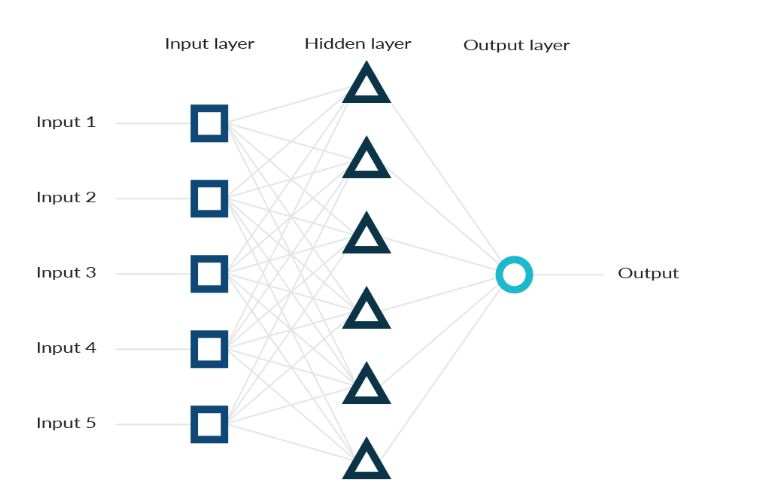
\includegraphics[scale=0.2]{figures/chapter-7-beda-deep-neu-dan-deep-learn-fadila.jpg}
\caption{Perbedaan Deep NW Dan Deep Learn- fadila}
\label{chapter-7-beda-deep-neu-dan-deep-learn-fadila}
\end{figure}
\par
\par
\end{itemize}
\par
\par
\item Bagaimana Perhitungan Algoritma Dengan Ukuran Stride (NPM mod3+1)x(NPM mod3+1) Yang  Terdapat Pada Max Pooling :
\begin{itemize}
\item Penjelasan :
\par
\par
\end{itemize}
\end{enumerate}

\section{Rahmi Roza-1164085}
\subsection{Teori}
\begin{enumerate}
\item Kenapa File Suara Harus Dilakukan Tokenizer
\begin{itemize}
\item Penjelasan: Untuk membedakan karakter-karakter tertentu dalam suatu teks dan juga sebagai pemisah kata atau bukan.Tokenizer dilakukan dengan cara melakukan pemotongan string input berdasarkan tiap kata yang menyusunnya.
\par 
\par
\item Ilustrasi Gambar
\item Tokenizer \ref{teori1}
\begin{figure}[!hbtp]
\centering
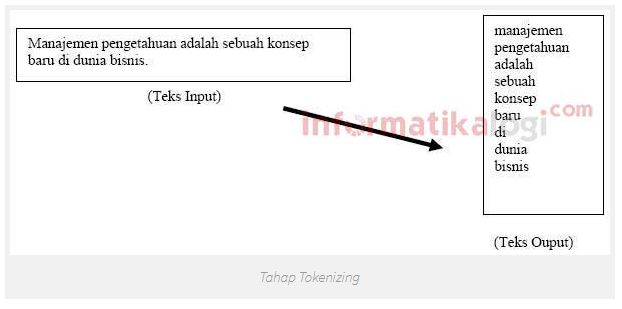
\includegraphics[scale=0.7]{figures/teori1.jpg}
\caption{Tokenizer Roza}
\label{teori1}
\end{figure}
\par
\end{itemize}
\par
\par

\item 	Apa Itu Deep Learning
\begin{itemize}
\item Penjelasan: 
\par  Deep learning merupakan sub bidang pembelajaran mesin yang berkaitan dengan algoritma.
\end{itemize}
\par
\par

\item Apa itu Deep Neural Network Dan Apa Bedanya Dengan Deep Learning :
\begin{itemize}
\item Penjelasan Deep Neural Network : 
\par  Deep neural network adalah jaringan syaraf dengan tingkat kompleksitas tertentu, jaringan syaraf dengan lebih dari dua lapisan.
\par
\item Perbedaan Deep Neural Network Dan Deep Learning :
\par Perbedaan antara deep neural network dan deep learning terletak pada kedalaman model. deep learning adalah frasa yang digunakan untuk jaringan saraf yang kompleks. Kompleksitas ini disebabkan oleh pola yang rumit tentang bagaimana informasi dapat mengalir di seluruh model.
\end{itemize}
\par
\par

\end{enumerate}